%%\chapter{Processes}
% \label{chapter-scenario-processes}

\section{Simple Process Sequence}

\textbf{Created by:} Jim Logan \\
\textbf{Modified by:} Jim Logan \\

\subsection*{Scenario Objective}
% Instruction box
This scenario demonstrates how to represent a sequence of time-stamped events using the \textbf{BFO/IOF ontology}. Several use cases are given, where each subsequent use case augments the previous one, culminating in a use case that demonstrates how to determine the type of an overall process automatically from a sequence of sub-processes.

\textit{ 
Note: I'm unsure what to say about the purpose of doing this!
}

\subsection*{General Pattern Description}

This pattern creates several instances of \cname{bfo}{process}. Each such \cname{bfo}{process}
\opname{core}{occupiesTemporalRegion}
one
\cname{bfo}{temporalInterval}
with single start and end instances of
\cname{bfo}{TemporalInstant}.
Each such \cname{bfo}{TemporalInstant}
\opname{core}{hasValueExpressionAtAllTimes} some
\cname{core}{TemporalInstantValueExpression}, according to the earlier pattern in
\ref{sec-clock-calendar}.

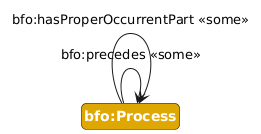
\includegraphics[scale=0.5]{scenarios/simple-process-sequence/image/general-pattern.png}


\subsection*{Use Case: Simple Process Sequence}\label{SimpleProcessSequence}
This first use case is the simplest. It uses the example data, shown below, to create corresponding instances in the IOF theory of what must have existed in the world to justify the data.

 \textit{ 
Describe a concrete use case for the pattern. (Multiple use cases can be described for one pattern. If multiple, please use distinct use case titles and repeat all subsubsections for each use case.)
  }

\newcommand{\ti}{\cname{bfo}{TemporalInstant }}

\subsubsection*{Use-Case Pattern Description}
This use case follows the pattern in \ref{sec-clock-calendar}.
Each timestamp in a row that is marked "Start" creates several instances at once and then wires them together as follows:
a \cname{bfo}{Process} that \opname{core}{occupiesTemporalRegion} a \ti that \opname{bfo}{hasFirstInstant} a \cname{bfo}{TemporalInstant} that \cname{iof}{hasValueExpressionAtAllTimes} a \cname{time}{DateTimeDescription}.

Note that in this first use case, the EventType is used to create a generic \cname{bfo}{process}. A subsequent use case will create an instance of a more specific type of process that corresponds to the EventType.

Each timestamp in a row that is marked "Stop" augments what was already created for a "Start" row with several more instances, and then wires them together as follows:
the already-created \cname{bfo}{TemporalRegion} \opname{bfo}{hasLastInstant} a \cname{bfo}{TemporalInstant} that \cname{iof}{hasValueExpressionAtAllTimes} a \cname{time}{DateTimeDescription}.

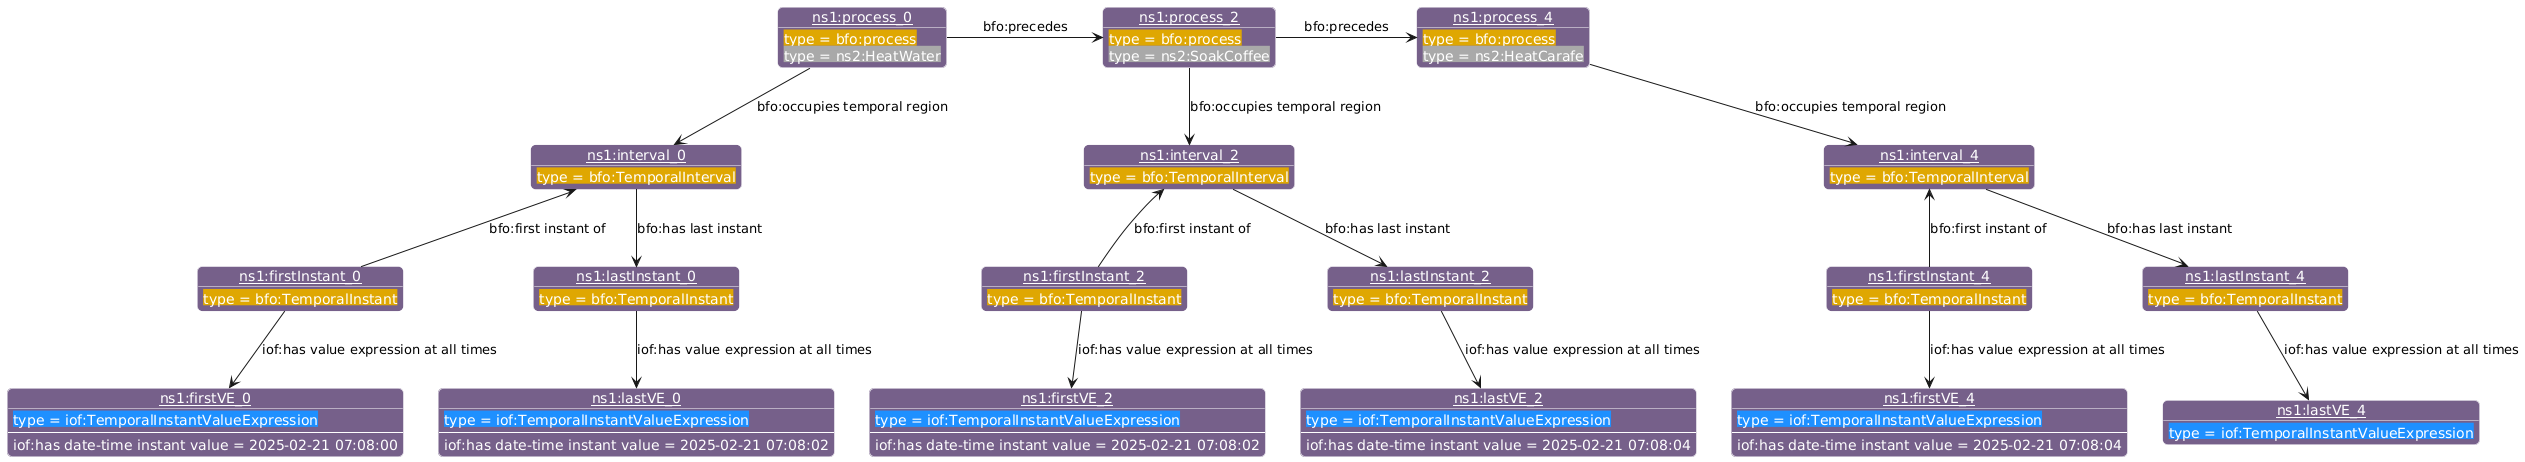
\includegraphics[scale=0.175]{scenarios/simple-process-sequence/image/instances.rdf.png}

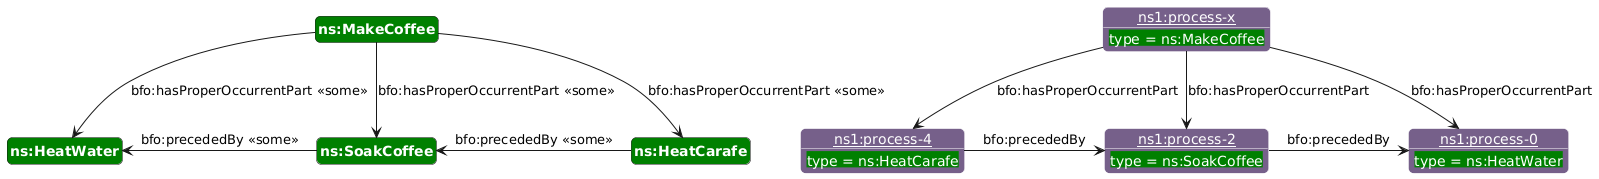
\includegraphics[scale=0.28]{scenarios/simple-process-sequence/image/advanced-instances.rdf.png}

% \textit{ 
%Provide a diagram which matches the use-case pattern description. \\
%\noindent \textit{This diagram is generally an object diagram. Please see examples of object diagram here.}
%  }

% \textit{ 
%Describe how the general pattern is applied to the use case. It is important to highlight within the description how the use-case-specific concepts align with the general pattern (e.g., SubClassOf Class for general pattern).
%  }

\subsubsection*{Use-Case Example Data}
The following table shows CSV data resulting from a fictitious machine that makes drip coffee. Each row contains the date and time at which an instance of a type of process started or stopped.

\begin{table}[ht]
    \centering
    \csvautotabular{scenarios/simple-process-sequence/data/EventLog.csv}
    \caption{An Example Event Log for Making Drip Coffee}
    \label{tab:DripCoffee}
\end{table}    

\subsubsection*{Data Mapping}
The following SPARQL converts the CSV file into RDF triples. Its WHERE clause connects to a service that makes each row in the CSV file available, it binds each CSV field to a variable, and constructs an IRI from a universally unique identifier (UUID). Its INSERT clause then uses those variables from a row in the CSV file to insert a pattern of three triples into a repository. The predicates of those triples exist to connect the IRI (bound to the variable "?id") to the three fields of each row.

% \lstinputlisting[language=sparql]{scenarios/simple-process-sequence/data/csv2rdf.rq}

\begin{verbatim}
INSERT {
    ?id ex:rowNumber ?rowNumber ;
        ex:timestamp ?Timestamp ;
        ex:eventType ?EventType ;
        ex:startStop ?StartStop .
}
WHERE {
  SERVICE <http://example.com/repositories/ontorefine:XXXXXXX> {
    BIND(?row_index as ?rowNumber) .
    BIND(xsd:dateTime(?c_Timestamp) as ?Timestamp) .
    BIND( ?c_EventType AS ?EventType ) .
    BIND( ?c_StartStop AS ?StartStop ) .
    BIND(IRI(CONCAT("https://ontogenesis-solutions.com/ontologies/examples/instances/row_", STR(?rowNumber))) AS ?id)
  }
}
\end{verbatim}

After the content of the CSV file is inserted into the triple store, the next SPARQL query pairs up the start and end of each type of event and then properly instantiates classes and properties from the IOF Core ontology. The syntax here demonstrates what may be a more familiar variable notation for some practitioners.

Note that the last row of the CSV file (shown in \ref{tab:DripCoffee}) has no "Stop" row because the drip coffee maker continues to heat the carafe until it is turned off, which, in this fictitious model, also disconnects power from the internal computer producing the event file. The SPARQL query handles this using an "OPTIONAL" clause.

Given a pattern match in the "WHERE" clause, all of the variables are ready for the "CONSTRUCT" clause.

% \lstinputlisting[language=sparql]{scenarios/simple-process-sequence/data/instances.rq}

\begin{verbatim}
CONSTRUCT {
    $process rdf:type bfo:BFO_0000015, $class ;     # Process            
             bfo:BFO_0000199 $interval . # occupiesTemporalRegion
    $interval rdf:type bfo:BFO_0000202 ;      # Temporal Interval
              bfo:BFO_0000222 $firstInstant ; # hasFirstInstant
              bfo:BFO_0000224 $lastInstant .  # hasLastInstant
    $firstInstant rdf:type bfo:BFO_0000203 ;      # Temporal Instant
                  iof-core:hasValueExpressionAtAllTimes $firstVE.
    $lastInstant rdf:type bfo:BFO_0000203 ;      # Temporal Instant
                 iof-core:hasValueExpressionAtAllTimes $lastVE .
    $firstVE rdf:type iof-core:TemporalInstantValueExpression ;
             iof-core:hasDateTimeInstantValue $startTime .
    $lastVE rdf:type iof-core:TemporalInstantValueExpression ;
            iof-core:hasDateTimeInstantValue $endTime .
}
WHERE {
    $startId ex:rowNumber $rowNumber ;
             ex:startStop "Start" ;
             ex:eventType $eventType ;
             ex:timestamp $startTime .
    OPTIONAL {
        $endId ex:startStop "Stop" ;
               ex:eventType $eventType ;
               ex:timestamp $endTime .
    }
    BIND(STR(inst:) AS $inst)
    BIND(STR($rowNumber) AS $rowNumberString)
    BIND(IRI(CONCAT($inst, "process_",      $rowNumberString)) AS $process)
    BIND(IRI(CONCAT($inst, "interval_",     $rowNumberString)) AS $interval)
    BIND(IRI(CONCAT($inst, "firstInstant_", $rowNumberString)) AS $firstInstant)
    BIND(IRI(CONCAT($inst, "lastInstant_",  $rowNumberString)) AS $lastInstant)
    BIND(IRI(CONCAT($inst, "firstVE_",      $rowNumberString)) AS $firstVE)
    BIND(IRI(CONCAT($inst, "lastVE_",       $rowNumberString)) AS $lastVE)
    BIND(STR(classes:) AS $classes)
    BIND(IRI(CONCAT($classes, $eventType)) AS $class)
}
\end{verbatim}




\begin{comment}
\subsubsection*{Data Validation}
 \textit{ 
Data validation can be performed in two ways: accessing interesting facts using SPARQL or validating whether the entire data conforms to the ontology using SHACL. It is preferable to provide both. \\
Provide the SPARQL query in the code block along with the result of the query. \\
  }

\subsection*{Use Case: Typed Process Sequence}
This use case extends the use case from section \ref{SimpleProcessSequence} with specializations of \cname{bfo}{process} corresponding to the EventType column in Table \ref{tab:DripCoffee}.

 \textit{ 
Describe a concrete use case for the pattern. (Multiple use cases can be described for one pattern. If multiple, please use distinct use case titles and repeat all subsubsections for each use case.)
  }

\subsubsection*{Use-Case Pattern Description}
 \textit{ 
Provide a diagram which matches the use-case pattern description. \\
\noindent \textit{This diagram is generally an object diagram. Please see examples of object diagram here.}
  }

 \textit{ 
Describe how the general pattern is applied to the use case. It is important to highlight within the description how the use-case-specific concepts align with the general pattern (e.g., SubClassOf Class for general pattern).
  }

\subsubsection*{Use-Case Example Data}
The following table shows CSV data resulting from a fictitious machine that makes drip coffee. Each row contains the date and time at which a type of event started or stopped.


\subsubsection*{Data Mapping}
 \textit{ 
Describe how the data was mapped to RDF. Provide an INSERT DATA/ INSERT SPARQL for mapping. Use INSERT only when the use case example data needs further manipulation. \\
For INSERT DATA SPARQL, use only 2/3 records/transactions with named class and individuals. \\
For INSERT SPARQL, declare column names by `\{ \}' to the variable.  
For INSERT query, 
For both, do not use blank nodes.    
  }

\subsubsection*{Data Validation}
 \textit{ 
Data validation can be performed in two ways: accessing interesting facts using SPARQL or validating whether the entire data conforms to the ontology using SHACL. It is preferable to provide both. \\
Provide the SPARQL query in the code block along with the result of the query. \\
  }    
\end{comment}